\lecture{Задача локализации точки 2}{Виталий Дьячков}

\subsection{Введение}

Поиск в простейшей абстрактной форме можно представить следующим образом: есть некоторый \textbf{набор данных} и некоторый \textbf{новый элемент данных}. Поиск – это установление связи между новым элементом данных и набором данных. Среди всех форм поиска можно выделить геометрическую форму. Это обусловлено тем, что в геометрических приложениях наборы данных представляют собой сложные структуры, такие как многоугольники, графы и т.п., а в качестве новых элементов данных могут использоваться точки, регионы и т.п.

В дальнейшем, поисковое сообщение, в соответствии с которым ведется просмотр набора данных, будем называть запросом. От типа набора данных, то есть от структур в нем содержащихся, и от набора допустимых запросов будет сильно зависеть организация набора данных и алгоритмы обработки последних. Важность этого аспекта задачи поиска поясним на простом примере. Пусть имеется массив чисел и требуется узнать, содержит ли этот массив некоторое заданное число. Когда такой вопрос возникает единожды, то можно получить ответ на него, просмотрев весь массив, то есть затратив время, пропорциональное размеру массива. В этом случае было бы неразумно затрачивать время на предобработку в надежде ускорить прохождение последующих запросов. Запросы такого типа будем называть уникальными. Однако могут быть запросы, обработка которых повторяется многократно на одном и том же массиве. Такие запросы будем называть массовыми. В последнем случае стоит отсортировать массив, затратив на это некоторое время. Это позволит отвечать на запрос за время, пропорциональное логарифму размера массива.

В связи с этим анализ геометрических алгоритмов поиска следует сосредоточить на трех следующих направлениях:
\begin{itemize}
    \item \textbf{время предобработки} --- cколько времени необходимо для организации данных перед поиском;
    \item \textbf{время запроса} -- cколько времени необходимо для ответа на один запрос;
    \item \textbf{память} --- cколько памяти необходимо для структуры данных;
\end{itemize}

\subsection{Задача локализации точки}
Одной из главных моделей геометрического поиска является задача локализации нового элемента, когда набор данных представляет собой разбиение геометрического пространства на области, а новый элемент данных является новым элементом. Локализация состоит в определении области, содержащей запрошенный новый элемент.

Трудоемкость этой задачи существенно зависит от природы пространства и от способа его разбиения.

Простыми словами:
У нас есть несколько многоугольников, и нам надо относительно быстро отвечать какому многоугольнику принадлежит точка

\textbf{Определение.} \textit{Плоским прямолинейным графом $G$ будем называть двойку объектов ($V,E$), где $V$ --- множество точек на плоскости (вершин графа), а $E$ --- множество непересекающихся отрезков (ребер графа), концами которых являются точки из множества $E$.}

\textbf{Определение.} \textit{Локализацией точки на планарном подразбиении будем называть процесс определения области, содержащей запрошенную точку.}

Чтобы вести поиск на планарном подразбиении, можно попытаться на этапе предобработки произвести декомпозицию исходных областей на такие области, для которых поисковая операция относительно проста (например треугольники или трапеции). Тогда успех в локализации точки зависит от возможности быстро сузить множество компонент декомпозиции, которые следует просмотреть. Из всего этого следует, что главная идея заключается в преобразовании исходных областей в новые геометрические объекты, допускающие двоичный поиск.

\subsection{Методы}

Давайте рассмотрим некоторые методы.
\subsubsection*{Метод полос}

Пусть задан ППЛГ $G$. Проведем горизонтальные прямые через каждую его вершину (см. Рис.1.). Если граф содержит $N$ вершин, то эти горизонтальные прямые разделяют плоскость на $N+1$ полосу.

\begin{figure}[H]
    \centering
    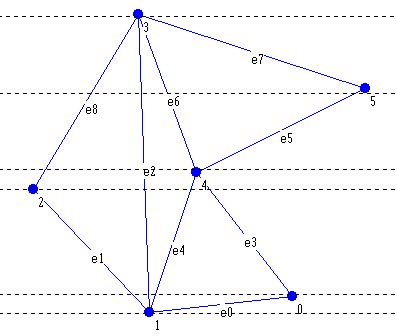
\includegraphics[width=0.6\linewidth]{polos.png}
    \caption{Метод полос}
\end{figure}

Если провести сортировку этих полос по ординате, то появится возможность найти ту полосу, в которой лежит пробная точка, за время $O$($logN$).

Пересечение одной из полос с графом $G$ состоит из ребер этого графа или их фрагментов, определяющих трапеции. Такие трапеции, очевидно, могут вырождаться в треугольники. Ключом к алгоритму локализации точки является то, что ребра графа внутри полосы не пересекаются между собой. Поэтому их можно полностью упорядочить слева направо и использовать двоичный поиск для определения той трапеции, которая содержит запрошенную точку.

Итак, поиск состоит из двух последовательно выполняемых шагов:
\begin{enumerate}
    \item Определение полосы содержащей точку.
    \item Определение трапеции.
\end{enumerate}

Оба шага требуют в худшем случае времени $O$($logN$), а значит время запроса в худшем случае равно $O$($logN$). \\
Время предобработки: $O$($N^2$) \\
Память: $O$($N^2$)

\subsubsection*{Метод цепей}
\par Для начала нам надо ввести понятие цепи \\
\textbf{Определение.} \textit{Цепью $C = $ {$v_1, v_2,...,v_n$} называется ППЛГ с вершинами {$v_1, v_2,...,v_n$} и ребрами \\{${v_i,v_{i+1}:=1,...,N-1}$}} \\
Метод цепей для локализации точки заключается в следующем:
\begin{enumerate}
    \item Предварительная обработка
          \begin{itemize}
              \item Упорядочиваем ребра планарного разбиения в виде цепей. Цепь --- это последовательность ребер, которые идут слева направо (или сверху вниз).
              \item Строим структуру данных для быстрого поиска нужной цепи.
          \end{itemize}
    \item Локализация точки
          \begin{itemize}
              \item Сначала, используя структуру данных, определяем цепь, которая находится над или под точкой.
              \item Затем, двоичным поиском по ребрам в цепи, находим грань, в которой находится точка.
          \end{itemize}
\end{enumerate}

\begin{figure}[H]
    \centering
    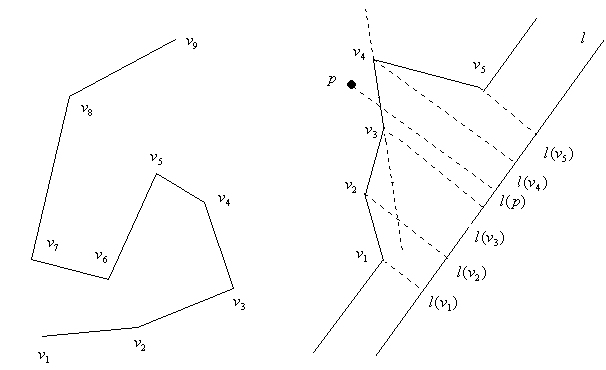
\includegraphics[width=0.6\linewidth]{cep.png}
    \caption{Примеры цепей: слева – общего вида; справа – монотонная по отношению к прямой $l$}
\end{figure}
Оценим этот метод: \\
Время предобработки: $O$($NlogN$) в худшем случае,  или $O$($n$) усредненно \\
Время запроса    $O$($logN$) \\
Память        $O$($n$)

\subsubsection*{Метод триангуляции}

\par В контексте планарных разбиений, триангуляция – это процесс разделения многоугольной области (или плоскости, содержащей многоугольные области) на треугольники. Другими словами, это разбиение плоскости на треугольники, используя заданные вершины и, возможно, добавляя новые вершины. Важно, что полученные треугольники не перекрываются и их объединение покрывает исходную область. Есть разные способы триангуляции.
\par В итоге, мы разбиваем плоскость на треугольники и локализуем точку. Давайте оценим этот алгоритм: \\
Время предобработки:  $O$($NlogN$) \\
Время запроса :  $O$($N$) в лучшем случае, когда накладываем ограничения, то $O$($NlogN$)  \\
Память : $O$($n$)

Более подробный разбор триангуляции Делоне будет в следующей лекции.
